\documentclass[border=2pt]{standalone}
\usepackage{pgfplots}
\pgfplotsset{compat=1.18}
\begin{document}
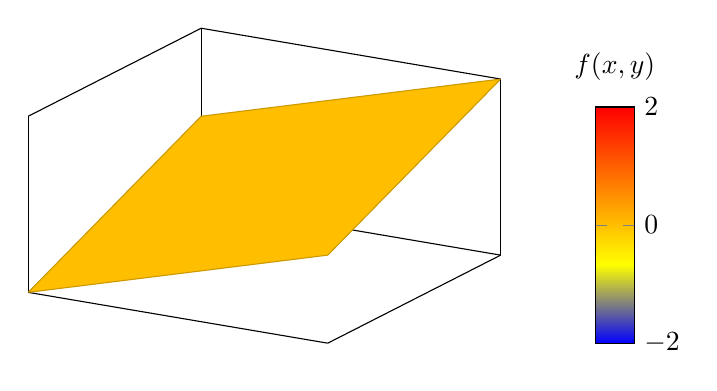
\begin{tikzpicture}
\begin{axis}[scale only axis,width=6cm,height=4cm,view={30}{30},
  enlargelimits=false,xmin=-1,xmax=1,ymin=-1,ymax=1,zmin=-2,zmax=2,
  xtick=\empty,ytick=\empty,ztick=\empty,colorbar,
  colorbar style={at={(1.2,0)},anchor=south west,width=.5cm,height=3cm,
    ytick={-2,0,2},title={$f(x,y)$}}]
\addplot3[surf,samples=2,domain=-1:1,y domain=-1:1] {x+y};
\end{axis}
\end{tikzpicture}
\end{document}
